\section{Usability}
\label{sub:usability}

Usability can be defined as \enquote{when a product or service is truly usable, the user can do what he or she wants to do, the way he or she expects to be able to do it, without hindrance, hesitation, or questions}~\cite{RubinChisnellSpool08}.

There are different ways of evaluating the usability of a product. The two, being looked at in this report, are \textit{empirical} and \textit{heuristic} testing. The goal of a usability test is to come up with a list of usability problems. A usability problem is a deficiency in a product that makes it less usable. An example of a usability problem is when a simple task like deleting an email takes an inappropriate amount of effort.

\subsection{Usability Testing}
\label{sub:usabilityTesting}
Usability testing is an empirical technique used to evaluate a product by testing it with users in focus. The purpose of the test is to determine usability problems with the product~\cite{RubinChisnellSpool08}. In this report the term \emph{usability testing} is used to refer to the process of testing with users, and not as a general term for testing usability. The test is intended to be realistic and simulate potential scenarios that can happen while using the product. A usability test is usually performed with a representative user performing a series of tasks. A test monitor will watch the participant completing the tasks without interrupting the participant in doing the tasks. While the participant is solving the task, a data logger is noting how the participant is solving the tasks given and the problems faced doing so.

After a usability test is conducted, the results must be analysed and documented. In most usability testing analysis methods, this involves spending a lot of time doing video data analysis. In this project, a newer method called \enquote{Instant Data Analysis} (IDA)~\cite{kjeldskov2004instant} was used. This method seeks to reduce the resources required to conduct the analysis. In IDA the procedure is as follows. After the test, a one hour brainstorm session between the data logger and test monitor has to occur. A facilitator manages the brainstorm and writes usability problems on a whiteboard. After the brainstorm, the facilitator spends 1-1.5 hours writing usability problems into a ranked list. Using IDA reduces the time to do analysis to 10\% of the traditional video analysis~\cite{kjeldskov2004instant}. While still finding 85\% of the critical problems.

\subsection{Heuristic Evaluation}
Heuristic evaluation is a method to inspect usability of computer
software. It involves a number of evaluators that are presented with
an interface design and asked to comment on it. This is used to come
up with a list of usability problems in a user interface design. This
information can be used as part of an iterative design process to make the design more usable. Heuristic evaluation is a cheap and intuitive way of doing usability evaluation and it does not require advanced planning~\cite{Nielsen1990}.

Heuristic evaluation is usually done by judging how the software meets certain predetermined heuristics.~\cite{Nielsen1990} introduced a set of ten heuristics that was then later updated in~\cite{Nielsen1994}, that are as follows:

\begin{enumerate}
  \item Visibility of system status
  \item Match between system and the real world
  \item User control and freedom
  \item Consistency and standards
  \item Error prevention
  \item Recognition rather than recall
  \item Flexibility and efficiency of use
  \item Aesthetic and minimalist design
  \item Help users recognise, diagnose, and recover from errors
  \item Help and documentation
\end{enumerate}

The method is not good for finding all problems; an individual person can only find between 20\% and 51\% of all problems~\cite{Nielsen1990}. Therefore it is recommended that multiple people conduct the evaluation independently of one another. The results can then be merged together.~\cite{Nielsen1990} recommends that 3 to 5 people do independent evaluation to get good coverage.

A disadvantage of heuristic evaluation is that it sometimes identifies usability problems without providing direct suggestions for how to solve them~\cite{Nielsen1990}. The method is biased by the current mindset of the evaluators and normally does not generate breakthroughs in the evaluated design.

\section{Usability Test in Laboratory}
Usability testing in this project will be used as a tool to test and
ensure quality of the user interface of the client application. An empirical evaluation was chosen over heuristic evaluation since it would get more data on usability problems. It would also evaluate the program with potential users, this would give assurance that the program lives up to the users' expectation and requirements. The tests will be performed on
typical users that were determined in \cref{userInterviews}, who are
representative end users of the product. It was chosen to conduct the
test in a laboratory since it is easy to create a controllable
environment and record video. Because of the limited time, it was
chosen to do IDA as described in \cref{sub:usabilityTesting}. According to \cite{kjeldskov2004instant} this will not find as many usability problems as video analysis. But it will only take 10\% of the time.

\subsection{Procedure}
\begin{figure}[hbtp]
  \centering
  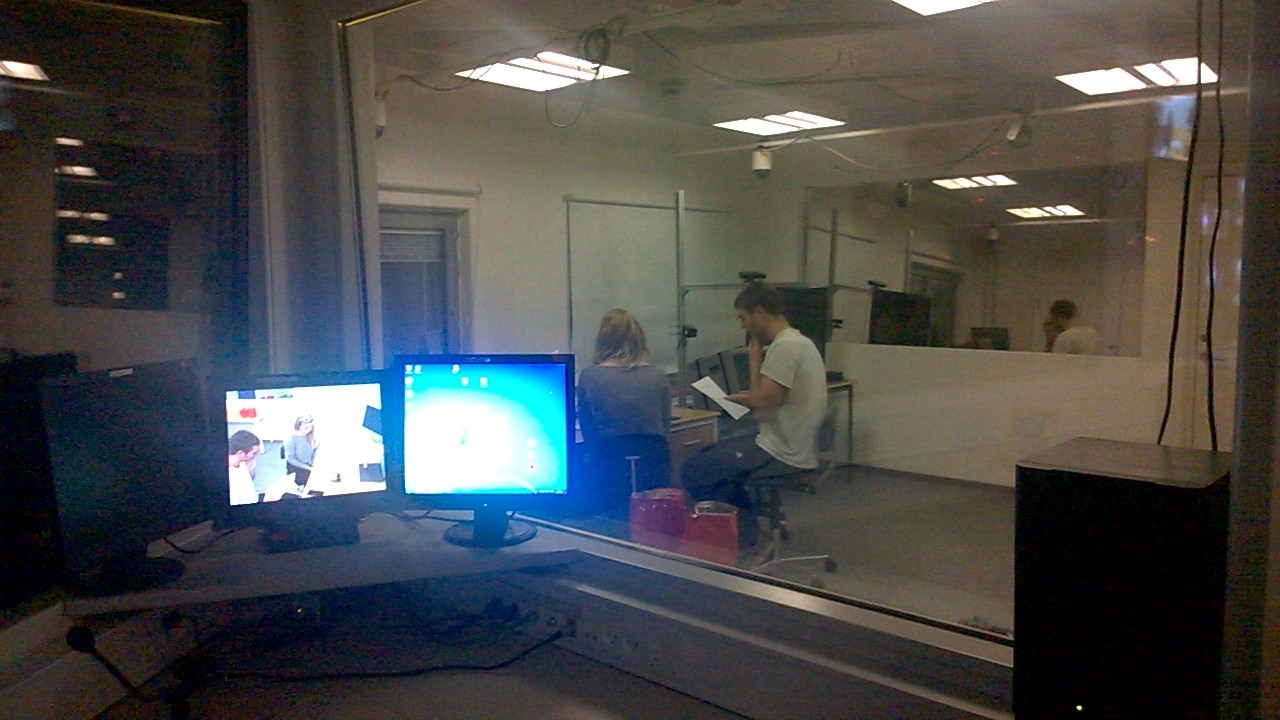
\includegraphics[width=1\linewidth]{subjectRoom}
  \caption{View from the control room into the subject room.}\label{fig:subjectRoom}
\end{figure}

The tests were conducted at the usability laboratory in the Department of Computer Science at Aalborg University. On \cref{fig:subjectRoom} is a picture of the usability laboratory. The laboratory is split into three different rooms: control room, subject room and observer room. The test was done on a smartphone of the model OnePlus One. This was the phone that was available at hand and it is equipped with a powerful processor. The members of the group were assigned different roles; two persons were assigned as alternating datalogger in the observer room and leader in the subject room. Another person was datalogger at all tests also in the observer room taking notes. A fourth person was responsible for entertaining the test subjects when they were not being tested and also driving the subjects that needed help arriving at the testing location. The fifth person was the video operator and was responsible for recording and mixing the video feeds from the subject room. The last person was assigned the role of social environment simulator. He was responsible for simulating other users actively using the test application, by adding multiple tracks to the playlist. This was done in order to make the usage of the application more realistic. The application tries to make a social experience and ideally there would be more than one person interacting with the server at a time. This tasks was though a fairly trivial task since all tracks and when to add them where decided before the tests. This last person therefore also acted as a datalogger most of the time.

The tests was done as think-aloud sessions. At the start of a test, an introduction was read out loud to the test
subject. The introduction can be found in
\cref{usabilityTestIntro}. The subject would then answer a
questionnaire which can be found in \cref{tab:participants}. The test
proceeded with the test subjects reading a premade task and then
trying to accomplish that task. All tasks can be seen in \cref{usability_tasks}. According to~\cite{RubinChisnellSpool08}, the task description has to be detailed enough, so that no excessive information about the test program is exposed. The tasks was designed to take about 15 min. After the tasks was completed there was extra time for a free-form discussion about the application. In the end each test ended up taking 15 to 30 min. This difference in time came mainly from the free-form discussion.

\subsection{Participants}
It was decided to test with users, because it would give an indication
of how real end-users use the system. Since the system is to be used
in a bar and is targeted for students, students were chosen as test
subjects. The subjects were recruited from the user interviews
described in \cref{userInterviews}. \Cref{tab:participants} presents
information gathered from the before mentioned questionnaire.

\begin{table}[hbtp]
    \centering
    \tabcolsep=0.10cm
    \begin{tabular}{lccccr}
        \toprule
        \textbf{\#} & \textbf{Sex} & \textbf{Age} & \textbf{Field of study} &
        \textbf{Smartphone experience} & \textbf{Primary phone} \\
        \midrule
        1                   & F               & 20           & Techno-Anthropology       & Experienced                    & iOS                    \\
        2                   & F               & 19           & Mathematics             & Intermediate                   & Android, iOS           \\
        3                   & F               & 20           & SIV Spanish             & Experienced                    & iOS                    \\
        4                   & F               & 22           & Electronics and IT      & Intermediate                   & Android                \\
        5                   & M               & 20           & Electronics and
        IT      & Experienced                    & Android                \\
        \bottomrule
    \end{tabular}
    \caption{Participants}\label{tab:participants}
\end{table}

\subsection{Data Collection}
The screen of the phone was recorded with software on the phone. The
video feeds from the two cameras in the test room were recorded to a
DVD. The data logger was taking notes while the test subjects were
performing their tasks.

\subsection{Data Analysis}
It was not possible to conduct the IDA brainstorming and data analysis sessions the same day as the tests, since the subjects where only able to conduct testing after normal working hours, and it would be too late in the evening after the tests, to ensure a good quality of the sessions. This presented a problem, since IDA normally requires these sessions, to be done on the same day as the test. Since it was not possible to move the tests, it was decided to compensate for this with multiple dataloggers. Normally IDA only requires one person to be assigned as a datalogger. In the tests conducted two people would at any time be dedicated dataloggers. The environment simulator would furthermore, most of the time, also act as a datalogger, resulting in 2-3 dataloggers during the tests. It was assessed that this would be enough, to compensate for the brainstorm and data analysis sessions delay. The session where conducted the first thing in the morning the next day. \jenote{Ret dette afsnit igennem}

The data analysis can be split into four different areas; brainstorm, task review, note review and severity rating. These four areas where created according to the the analysis part of IDA~\cite{Kjeldskov2004}.

\subsubsection{Brainstorm}
First the brainstorm session where conducted. During the brainstorm session one person was assigned the role of IDA facilitator. Everyone in the group thereafter stated all problems found during the tests they could find from memory.

\subsubsection{Task review}
After the brainstorm the task review session where conducted. Here the tasks where taken in use for remembering additional problems for specific tasks. The IDA facilitator where responsible reading the questions aloud and writing down every problem found, convertinf these with problems found in the brainstorm.

\subsubsection{Note review}
In the note review session the notes taken by the dataloggers where taken in use. Here the IDA facilitator converted the notes taken by the dataloggers to problems and combined, if possible, these whith already stated problems. This where done in collaboration with the rest of the group to ensure everyone agreed and because these notes could trigger additional problems from memories. All problems where written down.

\subsubsection{Severity rating}
During this session every problem found in the earlier sessions where discussed. Problems that could where organised into one general problem. Also if problems where a part of a problem chain, for instance if a person did not know how the 
 
After this the data was organized into a list of problems. The problems was identified into 3 different categories from \cite{molich2007usable}: minor, serious, or critical and ordere after this on the list. Minor problems is when the user hesitates or is delayed for a few minutes. Serious is if the user is delayed for more time or expresses irritation. Critical is when the user total stop and cannot process without human intervention.

In total the analysis lasted about 1½ hours. During the sessions screen recordings and the DVD was used during the analysis when there was confusion about what happened at the test. The result of the analysis was a written list of problems. The ranking of the problem, a problem description and which test persons suffered from the problem is noted.

\subsubsection{Serious}
\textbf{Problem \#1 - Vote confusion. The user does not know how votes work, what the person has voted for and when the person has voted. Test persons \#1, \#2, \#3, \#4 and \#5.}\\
All test persons were unsure how votes work. They did not receive any indication about how many votes they had. All of them were also not sure which track they had currently voted on. Also, no confirmation upon voting was displayed.\\

\noindent\textbf{Problem \#2 - Confusion about multiple copies of the same song on the playlist and now playing. Test persons \#2, \#4 and \#5.}\\
When in the playlist view, a track would both be contained in the playlist of the venue while at the same time being displayed as now playing. An example of this can be seen in \cref{fig:twoSongs}. This would confuse the test persons, and they would get unsure about which end of the playlist was ranked highest.\\

\begin{figure}[hbtp]
  \centering
  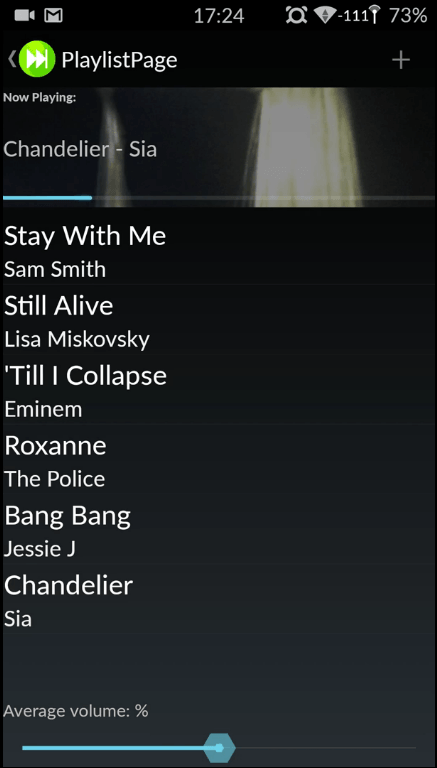
\includegraphics[width=0.3\linewidth]{twoSongs}
  \caption{Chandelier by Sia is displayed as currently playing, but is still at the bottom of the playlist.}\label{fig:twoSongs}
\end{figure}

\noindent\textbf{Problem \#3 - The user is confused on how well tracks are doing on the playlist. Test persons \#1, \#2 and \#5.}\\
This problem relates to problem \#2. There was no indication about how the tracks in the playlist are ordered. When asked about which track would be played next, some test persons had difficulties determining this.\\

\subsubsection{Minor}
\textbf{Problem \#4 - Missing confirmation when adding tracks on search. Test persons \#1, \#3, \#4 and \#5.}\\
When pressing on a track after searching for it, no feedback was given whether the track was successfully voted for. It was just marked blue as seen on \cref{fig:search}\\

\begin{figure}[hbtp]
  \centering
  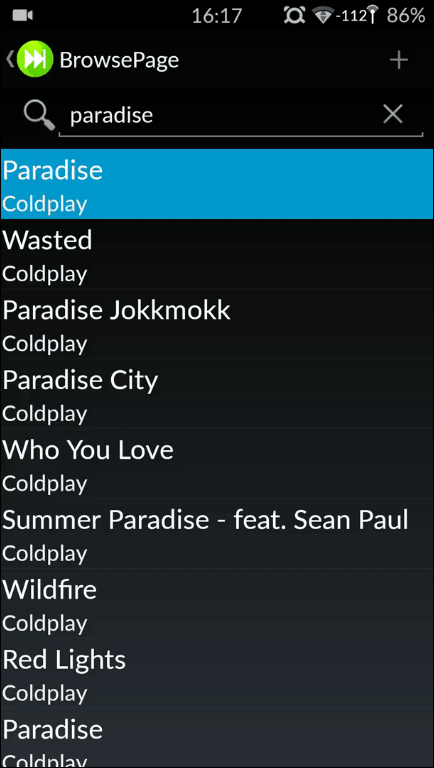
\includegraphics[width=0.3\linewidth]{search}
  \caption{When tapping a track on the search view to vote, the track
    would be marked blue, but no further indication of a successful
    vote would appear.}\label{fig:search}
\end{figure}

\noindent\textbf{Problem \#5 - Check-in confusion, does not know whether the person is checked
    in or not. Test persons \#1, \#2 and \#3.}\\
  When pressing on a venue to check in, test subjects would wait for
  something to happen in the app, even though the app was already
  checked in. There was no confirmation upon a successful check in.\\

\noindent\textbf{Problem \#6 - Did not know in which direction to swipe on the start page. Test
    persons \#2, \#4 and \#5.}\\
  When presented with the start page, a arrow and a corresponding text
  would indicate in which direction the test subject would have to
  swipe in order to get to the check in page. As seen in fig \cref{fig:swipe} this arrow was wrongly
  directed, which caused some test subjects to swipe in the wrong direction.\\

\begin{figure}[hbtp]
  \centering
  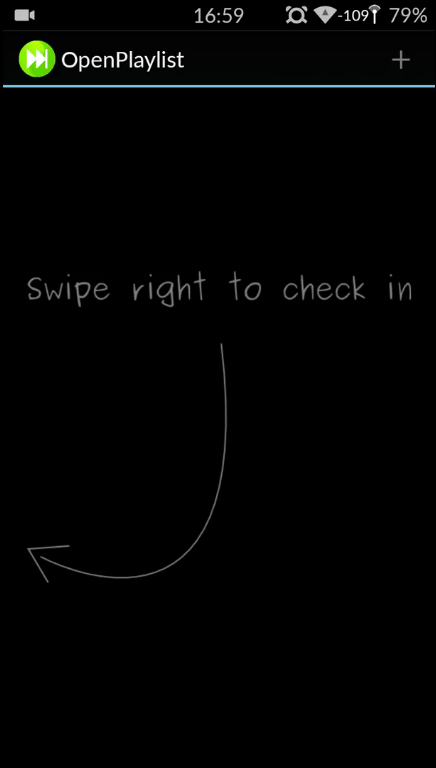
\includegraphics[width=0.3\linewidth]{swipe}
  \caption{Confusing arrow, which made some of the subject swipe in the wrong direction.}\label{fig:swipe}
\end{figure}

\noindent\textbf{Problem \#7 - Search confusion, does not know whether and when a search is
    happening. Test persons \#1 and \#5.}\\
  When pressing the search button, some feedback was given that the
  application was performing the search, but this was not standing out
  to the user. The user would therefore click twice on the search button.\\

\noindent\textbf{Problem \#8 - Loading indicator confuses user. They thought it was their actions
    that influenced the loading indicator. Test person \#2.}\\
  In the application, a automatic refresh of the playlist and
  now playing would update every 3 seconds. Whenever this automatic
  refresh happened, a small loading indicator would rotate. This
  indicator would show even if the user had not actively affected the application.\\

\noindent\textbf{Problem \#9 - Expected \enquote{clear search button}
  to remove results and bring user back to the playlist. Test person \#2.}\\
  When the test subject clicked on the clear button of the search bar,
  the subject was confused that just the text in the search bar was
  removed and not the search results. The subject described that it
  was expected to return back to the playlist.\\


\noindent\textbf{Problem \#10 - The IP-address in the venue page is
  confusing. They thought it was the number of guests at the venue. Test persons \#1 and \#2.}\\
  Some test subjects were confused about the number being displayed at
  the venue view as seen on \cref{fig:ip}. They were surprised as the number was rather big,
  e.g 192.168.1.10.\\

\begin{figure}[hbtp]
  \centering
  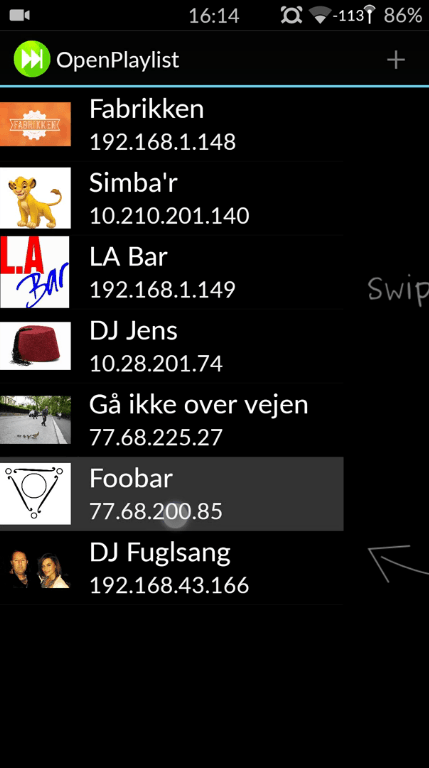
\includegraphics[width=0.3\linewidth]{ip}
  \caption{IP-address shown under each venue}\label{fig:ip}
\end{figure}

\noindent\textbf{Problem \#11 - Confusion about which votes were made by users and which were
    votes made by the bar. Test person \#2.}\\
  During the usability tests, an environment simulator would vote on
  songs. This affected the playlist being displayed on the test
  device. It was however unclear to the test subject that these votes
  were also user votes and not bar votes.\\

\noindent\textbf{Problem \#12 - Did not know what tracks in a search already existed on the
    playlist. Test person \#2.}\\
  When searching for tracks, no visual confirmation was given whether
  the searched track was already on the playlist.\\

\noindent\textbf{Problem \#13 - Was confused why the search did not
  clear when the user made a new search. Test person \#2.}\\
  When a new search was performed right after a previous search, the
  search results of the new search would only display when the search
  was complete. The test subject expected the previous search results
  to disappear when the new search was conducted.\\

\noindent\textbf{Problem \#14 - Excepted ability to get more info when interacting with all
    tracks. Test person \#5.}\\
  One test subject was several times trying to interact with the
  tracks on the playlist in order to get additional information. This
  feature was not implemented.

\subsection{Usability Test Summary}
As no critical problems were found in the use of the system and all participants were able to complete all the tasks. The usability of the system is concluded to be good, but certainly not perfect. The problems found can be discussed and eventually solved, leading to a more usable system.

It was decided to fix problem \#1, \#2, \#3, \#4, \#5, \#6 and
\#10. These problems were chosen to cover all serious problems and
some of the most common minor problems. The final version of the
client application had these problems fixed. After the fixes, a new test
could be conducted in order to confirm that the problems was indeed
fixed, but this was dropped due to time constraints.

While fixing problems \#4 and \#5, confirmation was added when adding
tracks from the search view and when checking into a venue. This results in a slightly different
interaction with the application, as the application will now forward
the user to a different screen upon adding tracks and checking into a venue.
